
\subsubsection{Confronto tra Attriti: Il Caso del Piano Inclinato}
In generale, la forza limite che separa lo stato di \textbf{QUIETE} (in cui agisce l'attrito statico $\vec{F}_s$) dallo stato di \textbf{MOTO} (in cui agisce l'attrito dinamico $\vec{F}_d$) corrisponde alla forza di attrito statico massima ($F_{s,max}$).

Consideriamo il caso generico di un corpo su un \textbf{piano inclinato} di un angolo $\theta$. Ci troviamo nella situazione limite in cui il corpo è sul punto di muoversi (imminente moto), quindi $F_s = F_{s,max} = \mu_s N$.

Scomponiamo le forze lungo gli assi:
\begin{itemize}
    \item Asse $x$ (parallelo al piano, verso il basso): componente parallela del peso $P_{\parallel}$ e attrito statico $F_s$.
    \item Asse $y$ (perpendicolare al piano): reazione vincolare $N$ e componente normale del peso $P_{\perp}$.
\end{itemize}

Il sistema all'equilibrio limite diventa:
\begin{equation}
\begin{cases}
    \sum F_x = m g \sin\theta - F_{s,max} = 0 \\
    \sum F_y = N - m g \cos\theta = 0
\end{cases}
\implies
\begin{cases}
    \mu_s N = m g \sin\theta \\
    N = m g \cos\theta
\end{cases}
\end{equation}

Sostituendo la seconda equazione nella prima:
\[ \mu_s (mg \cos\theta) = mg \sin\theta \]

Semplificando la massa $m$ e l'accelerazione $g$, otteniamo una relazione fondamentale:
\begin{equation}
    \mu_s = \frac{\sin\theta}{\cos\theta} = \tan\theta
\end{equation}

\paragraph{Angolo Critico ($\theta_{max}$)}
Ragionando all'opposto, possiamo calcolare l'angolo massimo di inclinazione $\theta_{max}$ per cui il corpo rimane fermo:
\[ \theta_{max} = \arctan(\mu_s) \]

\begin{itemize}
    \item Finché $\theta < \theta_{max}$: il corpo resta \textbf{fermo} ($F_s < F_{s,max}$).
    \item Quando $\theta > \theta_{max}$: la componente parallela del peso supera l'attrito massimo e il corpo \textbf{scivola}.
\end{itemize}

Geometricamente, questo definisce il cosiddetto \textbf{Cono di Attrito Statico}: se la risultante delle forze di contatto cade all'interno di questo cono di apertura $2\theta_{max}$, il corpo rimane in equilibrio.

\begin{figure}[h!]
    \centering
    \begin{minipage}{0.48\textwidth}
        \centering
        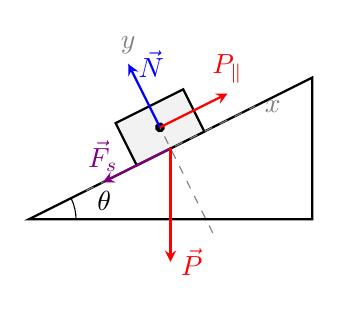
\begin{tikzpicture}[scale=1.2, >=stealth]
            % Piano Inclinato
            \coordinate (A) at (0,0);
            \coordinate (B) at (3,0);
            \coordinate (C) at (3,1.5); % tan(theta) = 0.5 -> theta approx 26.5 deg
            \draw[thick] (A) -- (B) -- (C) -- cycle;
            \draw (0.5,0) arc (0:26.5:0.5);
            \node at (0.8,0.2) {$\theta$};

            % Corpo
            \begin{scope}[shift={(1.5, 0.75)}, rotate=26.56]
                \draw[thick, fill=gray!10] (-0.4, 0) rectangle (0.4, 0.5);
                \fill (0, 0.25) circle (1.5pt); % Centro di massa

                % Sistema di riferimento locale
                \draw[gray, dashed] (-1,0) -- (1,0) node[right] {$x$};
                \draw[gray, dashed] (0,-1) -- (0,1) node[above] {$y$};

                % Forze
                \draw[->, thick, blue] (0, 0.25) -- (0, 1) node[right] {$\vec{N}$};
                \draw[->, thick, violet] (0, 0) -- (-0.8, 0) node[above] {$\vec{F}_{s}$};
                
                % Peso (non ruotato rispetto alla terra, ma scomposto qui)
                % Disegno le componenti per chiarezza
                \draw[->, thick, red] (0, 0.25) -- (0.8, 0.25) node[above] {$P_{\parallel}$}; % Sbagliato disegno vettoriale puro, meglio disegnare P verticale e scomporlo
            \end{scope}
            
            % Rifaccio Peso Verticale Reale
            \begin{scope}[shift={(1.5, 0.75)}]
                 \draw[->, thick, red] (0,0) -- (0,-1.2) node[right] {$\vec{P}$};
            \end{scope}
        \end{tikzpicture}
        \caption{Equilibrio su piano inclinato.}
    \end{minipage}
    \hfill
    \begin{minipage}{0.48\textwidth}
        \centering
        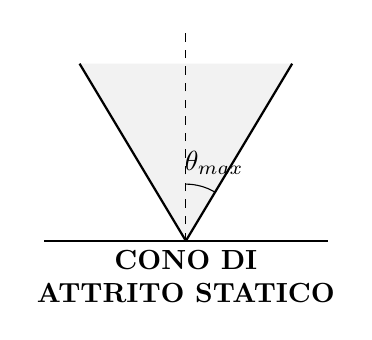
\begin{tikzpicture}[scale=0.9]
            % Piano
            \draw[thick] (-2,0) -- (2,0);
            % Cono
            \fill[gray!10] (0,0) -- (1.5, 2.5) -- (-1.5, 2.5) -- cycle;
            \draw[dashed] (0,0) -- (0,3);
            
            \draw[thick] (0,0) -- (1.5, 2.5);
            \draw[thick] (0,0) -- (-1.5, 2.5);
            
            % Angolo
            \draw (0,0.8) arc (90:59:0.8);
            \node at (0.4, 1.1) {$\theta_{max}$};
            
            \node[align=center, below] at (0,0) {\textbf{CONO DI}\\\textbf{ATTRITO STATICO}};
        \end{tikzpicture}
        \caption{Cono di Attrito.}
    \end{minipage}
\end{figure}

\paragraph{Nota sul piano orizzontale ($\theta = 0$):}
Su un piano orizzontale, in assenza di altre forze esterne, $P_{\parallel} = m g \sin(0) = 0$, quindi la forza di attrito necessaria per l'equilibrio è nulla.
Per misurare $\mu_s$ su un piano orizzontale, bisogna applicare una forza esterna $F_{min}$ finché il corpo non si stacca:
\[ F_{min} = |F_{s,max}| = \mu_s m g \implies \mu_s = \frac{F_{min}}{m g} \]
Dopo lo stacco, se vogliamo mantenere il corpo a velocità costante ($a=0$), dovremo applicare una forza pari all'attrito dinamico: $F_{motrice} = F_d = \mu_d m g$. Essendo solitamente $F_d < F_{s,max}$ (quindi $\mu_d < \mu_s$), la forza necessaria per mantenere il moto è minore di quella necessaria per avviarlo.
